\chapter{Verification of Attitude with a Camera}
\head{This is a description of a technique to verify an attitude
estimator by using a camera. It utilizes the horizon as the reference.}

\section{Objective}
To have a means to verify the attitude estimator, which is independent
of other inertial measurements.

\section{Method}
While testing it is of importance to make some verifications. When
implementing an attitude estimator for pitch and roll, it is hard to
verify whether it works as intended or not. A simple way to test it is
to put the sensor in positions that can be measured in a static
environment, that is by i.e. putting in on a table on what is to be
defined as flat, then angle it some known degrees and see if the
estimator agrees.

Depending on how exotic the estimator is, it might utilise a dynamic
model, in an attempt to improve the accuracy of the estimates. This is
harder to measure in the static lab setup. Another way is to record
the attitude with another setup that is known to work, but that could
not exist, hence the need to implement a new one. Alternatively a
method with a camera is proposed. This is the method to be described
in the following. This should provide a visual means of determining
the heading.

The idea here is to mount a camera on the rigid body object containing
the sensor in the longitudinal direction of the axis of interest. That
is a camera pointing forward for the roll determiniaton or a camera
pointing to one side for the pitch determiniaton. This is intended for
use on ships.

This method relies on a known reference, that is stationary or at least
known at all time. The most ideal scenario is to be in open water
where the horizon is between the sea and the sky. This is guaranteed
to be horizontal, giving us an absolute reference to compare against.

In a non ideal scenario is to e.g. use the harbour quay. This works if
the ship is not moving a lot around relative to the quay, else you
need to know the exact position to the quay to determine the angle the
camera should see as zero. This is also possible but is out of scope
of this description.

\begin{figure}[htbp]
\centering
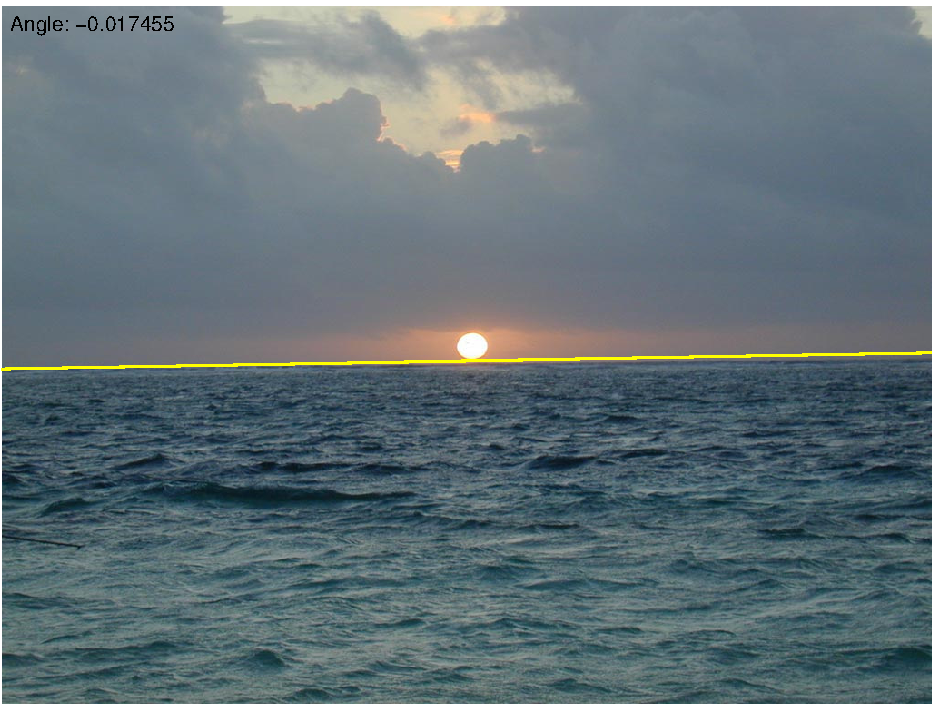
\includegraphics[width=\textwidth]{pdf/horizon}
\caption{Example plot of the angle calculated and overlaid on a frame
from the video recorded by the camera. The example image is fetched
from \citep{horizon-img}.}
\end{figure}

The idea is that the angle should be calculated from the image by some
means of image processing, but this has not been implemented, hence
there is not nice plot of this in action. 

When this is done it should be possible to get a time series of the
angles estimated from the image processing and compare it with the
time series from the observer on the same sea trail.
